\documentclass[tikz,border=15pt]{standalone}
\usepackage{tikz}
\usepackage{amsmath}
\usepackage{amssymb}
\usetikzlibrary{positioning, arrows.meta, calc, backgrounds, fit, shapes.geometric, decorations.pathreplacing, shadows}

\colorlet{color_intent}{blue!60!black}
\colorlet{color_slot}{green!50!black}
\colorlet{color_topic}{red!60!black}
\colorlet{color_shared}{black!70}

\begin{document}

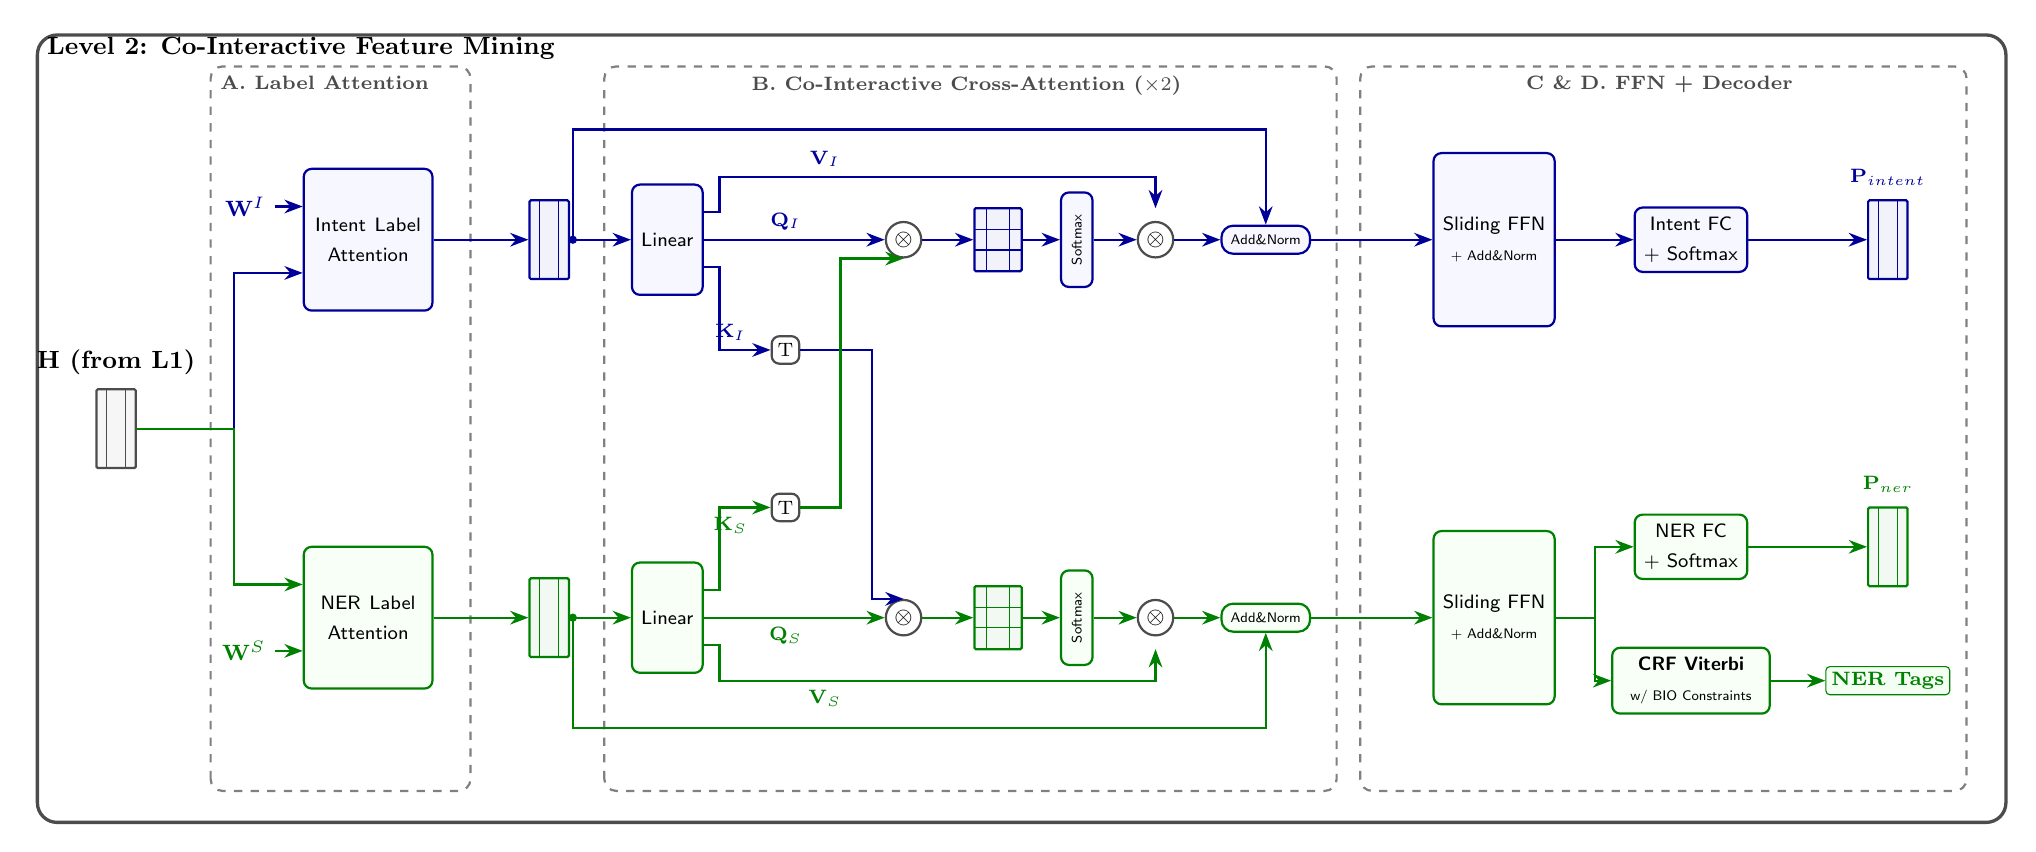
\begin{tikzpicture}[
    >=Stealth, font=\small\sffamily,
    color_intent/.style={blue!60!black},
    color_slot/.style={green!50!black},
    mainbox/.style={draw=black!70, rounded corners=2.5mm, line width=1.2pt},
    subbox/.style={draw=black!50, dashed, rounded corners=1.5mm, line width=0.8pt},
    block/.style={draw=black!70, fill=white, rounded corners=1mm, thick, align=center},
    intent_block/.style={block, draw=blue!60!black, fill=blue!3},
    slot_block/.style={block, draw=green!50!black, fill=green!3},
    op/.style={circle, draw=black!70, fill=white, inner sep=0.5pt, minimum size=0.45cm, thick, font=\footnotesize},
    arrow_intent/.style={->, thick, draw=blue!60!black},
    arrow_slot/.style={->, thick, draw=green!50!black},
    matrix_vert/.style={
        draw=#1, thick, fill=#1!5, minimum width=0.5cm, minimum height=1.0cm, rounded corners=0.5pt,
        path picture={
            \draw[#1, thin] (-0.12,-0.5) -- (-0.12,0.5);
            \draw[#1, thin] (0.12,-0.5) -- (0.12,0.5);
        }
    },
    matrix_grid/.style={
        draw=#1, thick, fill=#1!5, minimum width=0.6cm, minimum height=0.8cm, rounded corners=0.5pt,
        path picture={
            \draw[#1, thin] (-0.15,-0.4) -- (-0.15,0.4);
            \draw[#1, thin] (0.15,-0.4) -- (0.15,0.4);
            \draw[#1, thin] (-0.3,-0.13) -- (0.3,-0.13);
            \draw[#1, thin] (-0.3,0.13) -- (0.3,0.13);
        }
    }
]

% Kéo giãn mainbox để có thêm không gian đỉnh và đáy
\draw[mainbox] (-1.0, -5.0) rectangle (24.0, 5.0);
\node[anchor=north west, font=\bfseries] at (-1.0, 5.1) {\small{Level 2: Co-Interactive Feature Mining}};

% Input H
\node[matrix_vert=color_shared] (H_mat) at (0, 0) {};
\node[above=0.05cm of H_mat, font=\bfseries\small] {$\mathbf{H}$ (from L1)};

%% --- A. LABEL ATTENTION ---
\draw[subbox] (1.2, -4.6) rectangle (4.5, 4.6);
\node[anchor=north west, font=\bfseries\scriptsize, text=black!70] at (1.2, 4.6) {A. Label Attention};

\node[intent_block, minimum height=1.8cm, text width=1.4cm] (attn_I) at (3.2, 2.4) {\scriptsize Intent Label\\Attention};
\node[slot_block, minimum height=1.8cm, text width=1.4cm] (attn_S) at (3.2, -2.4) {\scriptsize NER Label\\Attention};

\node[font=\bfseries\footnotesize, text=color_intent, anchor=east] (WI) at ([xshift=-10pt, yshift=12pt]attn_I.west) {$\mathbf{W}^I$};
\node[font=\bfseries\footnotesize, text=color_slot, anchor=east] (WS) at ([xshift=-10pt, yshift=-12pt]attn_S.west) {$\mathbf{W}^S$};

\draw[arrow_intent] (WI.east) -- ([yshift=12pt]attn_I.west);
\draw[arrow_slot] (WS.east) -- ([yshift=-12pt]attn_S.west);
\draw[arrow_intent] (H_mat.east) -- (1.5, 0) |- ([yshift=-12pt]attn_I.west);
\draw[arrow_slot] (H_mat.east) -- (1.5, 0) |- ([yshift=12pt]attn_S.west);

\node[matrix_vert=color_intent] (mat_I1) at (5.5, 2.4) {};
\node[matrix_vert=color_slot] (mat_S1) at (5.5, -2.4) {};
\draw[arrow_intent] (attn_I.east) -- (mat_I1.west);
\draw[arrow_slot] (attn_S.east) -- (mat_S1.west);

%% --- B. CROSS ATTENTION ---
\draw[subbox] (6.2, -4.6) rectangle (15.5, 4.6);
\node[anchor=north, font=\bfseries\scriptsize, text=black!70] at (10.8, 4.6) {B. Co-Interactive Cross-Attention ($\times 2$)};

\node[intent_block, minimum height=1.4cm] (lin_I) at (7.0, 2.4) {\scriptsize Linear};
\node[slot_block, minimum height=1.4cm] (lin_S) at (7.0, -2.4) {\scriptsize Linear};
\draw[arrow_intent] (mat_I1.east) -- (lin_I.west);
\draw[arrow_slot] (mat_S1.east) -- (lin_S.west);

\node[op] (mul1_I) at (10.0, 2.4) {$\otimes$};
\node[op] (mul1_S) at (10.0, -2.4) {$\otimes$};
\node[block, minimum size=0.35cm, inner sep=1pt, font=\scriptsize] (T_I) at (8.5, 1.0) {T};
\node[block, minimum size=0.35cm, inner sep=1pt, font=\scriptsize] (T_S) at (8.5, -1.0) {T};

% -------------------------------------------------------------
% ROUTING CAO TỐC (ĐÃ ĐƯỢC QUY HOẠCH LẠI KHÔNG GIAN)
% -------------------------------------------------------------

% 1. Làn V_I: Cố định độ cao ở y = 3.2
\draw[arrow_intent] ([yshift=10pt]lin_I.east) -- ++(0.2,0) |- (13.2, 3.2) -- (13.2, 2.8);
\node[above, font=\scriptsize, text=color_intent] at (9.0, 3.2) {$\mathbf{V}_I$};

% 2. Làn Q_I: Đi thẳng ở y = 2.4
\draw[arrow_intent] (lin_I.east) -- (mul1_I.west); 
\node[above, font=\scriptsize, text=color_intent] at (8.5, 2.4) {$\mathbf{Q}_I$};

% 3. Làn K_I: Hạ xuống y = 1.0
\draw[arrow_intent] ([yshift=-10pt]lin_I.east) -- ++(0.2,0) |- (T_I.west); 
\node[above, font=\scriptsize, text=color_intent] at (7.8, 1.0) {$\mathbf{K}_I$};
\draw[arrow_intent] (T_I.east) -- (9.6, 1.0) |- (mul1_S.north);

% 4. Làn V_S: Cố định độ sâu ở y = -3.2
\draw[arrow_slot] ([yshift=-10pt]lin_S.east) -- ++(0.2,0) |- (13.2, -3.2) -- (13.2, -2.8);
\node[below, font=\scriptsize, text=color_slot] at (9.0, -3.2) {$\mathbf{V}_S$};

% 5. Làn Q_S: Đi thẳng ở y = -2.4
\draw[arrow_slot] (lin_S.east) -- (mul1_S.west); 
\node[below, font=\scriptsize, text=color_slot] at (8.5, -2.4) {$\mathbf{Q}_S$};

% 6. Làn K_S: Nâng lên y = -1.0
\draw[arrow_slot] ([yshift=10pt]lin_S.east) -- ++(0.2,0) |- (T_S.west); 
\node[below, font=\scriptsize, text=color_slot] at (7.8, -1.0) {$\mathbf{K}_S$};
\draw[arrow_slot] (T_S.east) -- (9.2, -1.0) |- (mul1_I.south);

% -------------------------------------------------------------
% PHẦN CÒN LẠI CỦA ATTENTION
% -------------------------------------------------------------
\node[matrix_grid=color_intent] (mat_I2) at (11.2, 2.4) {};
\node[intent_block, minimum height=1.2cm, minimum width=0.4cm] (soft_I) at (12.2, 2.4) {\rotatebox{90}{\tiny Softmax}};
\node[op] (mul2_I) at (13.2, 2.4) {$\otimes$};
\node[intent_block, rounded corners=1.5mm] (addnorm1_I) at (14.6, 2.4) {\tiny Add\&Norm};

\node[matrix_grid=color_slot] (mat_S2) at (11.2, -2.4) {};
\node[slot_block, minimum height=1.2cm, minimum width=0.4cm] (soft_S) at (12.2, -2.4) {\rotatebox{90}{\tiny Softmax}};
\node[op] (mul2_S) at (13.2, -2.4) {$\otimes$};
\node[slot_block, rounded corners=1.5mm] (addnorm1_S) at (14.6, -2.4) {\tiny Add\&Norm};

\draw[arrow_intent] (mul1_I.east) -- (mat_I2.west);
\draw[arrow_intent] (mat_I2.east) -- (soft_I.west);
\draw[arrow_intent] (soft_I.east) -- (mul2_I.west);
\draw[arrow_intent] (mul2_I.east) -- (addnorm1_I.west);

\draw[arrow_slot] (mul1_S.east) -- (mat_S2.west);
\draw[arrow_slot] (mat_S2.east) -- (soft_S.west);
\draw[arrow_slot] (soft_S.east) -- (mul2_S.west);
\draw[arrow_slot] (mul2_S.east) -- (addnorm1_S.west);

% 7. Đường Residual (Đã thêm node tròn đánh dấu và đẩy ra xa để không đè lên V)
\fill[color_intent] (5.8, 2.4) circle (1.5pt); % Nút giao Intent
\draw[arrow_intent] (5.8, 2.4) -- (5.8, 3.8) -| (addnorm1_I.north);

\fill[color_slot] (5.8, -2.4) circle (1.5pt); % Nút giao Slot
\draw[arrow_slot] (5.8, -2.4) -- (5.8, -3.8) -| (addnorm1_S.south);

%% --- C & D. FFN and DECODER ---
\draw[subbox] (15.8, -4.6) rectangle (23.5, 4.6);
\node[anchor=north, font=\bfseries\scriptsize, text=black!70] at (19.6, 4.6) {C \& D. FFN + Decoder};

\node[intent_block, minimum height=2.2cm, align=center] (ffn_I) at (17.5, 2.4) {\scriptsize Sliding FFN\\ \tiny + Add\&Norm};
\node[slot_block, minimum height=2.2cm, align=center] (ffn_S) at (17.5, -2.4) {\scriptsize Sliding FFN\\ \tiny + Add\&Norm};

\node[intent_block, align=center] (dec_I) at (20.0, 2.4) {\scriptsize Intent FC\\ \scriptsize + Softmax};
\node[slot_block, align=center] (dec_S) at (20.0, -1.5) {\scriptsize NER FC\\ \scriptsize + Softmax};
\node[slot_block, minimum width=2.0cm, align=center] (crf) at (20.0, -3.2) {\scriptsize \textbf{CRF Viterbi}\\ \tiny w/ BIO Constraints};

\draw[arrow_intent] (addnorm1_I.east) -- (ffn_I.west);
\draw[arrow_slot] (addnorm1_S.east) -- (ffn_S.west);
\draw[arrow_intent] (ffn_I.east) -- (dec_I.west);
\draw[arrow_slot] (ffn_S.east) -- ++(0.5,0) |- (dec_S.west);
\draw[arrow_slot] (ffn_S.east) -- ++(0.5,0) |- (crf.west);

\node[matrix_vert=color_intent] (P_I) at (22.5, 2.4) {}; \node[above=0.05cm of P_I, font=\bfseries\scriptsize, text=color_intent] {$\mathbf{P}_{intent}$};
\node[matrix_vert=color_slot] (P_S) at (22.5, -1.5) {}; \node[above=0.05cm of P_S, font=\bfseries\scriptsize, text=color_slot] {$\mathbf{P}_{ner}$};
\node[font=\scriptsize\bfseries, text=color_slot, fill=green!5, draw=green!50!black, rounded corners=0.5mm, inner sep=2pt] (ner_tags) at (22.5, -3.2) {NER Tags};

\draw[arrow_intent] (dec_I.east) -- (P_I.west);
\draw[arrow_slot] (dec_S.east) -- (P_S.west);
\draw[arrow_slot] (crf.east) -- (ner_tags.west);

\end{tikzpicture}

\end{document}